\subsection{Rigid bodies}
	To simulate the translational motion of a rigid body it is sufficient to simulate the motion of the center of gravity. As the vertices stay motionless relative to the center the position of every vertex can be calculated easily from the position of the center. 
	If the motion is arbitrary it can still be represented by just a translational and a rotational movement. 
	The simulation is done by a rigid body simulator. To simulate the body it stores the following parameters:
	\begin{itemize}
		\item densitiy $\rho$ and mass $m$
		\item the moment of inertia, which is constant to each body and behaves to rotational movement, as mass behaves to translational movement.
		\item linear position $\bm{x}$ and momentum $\bm{p}$
		\item orientation $\bm \Omega$ and angular momentum $\bm L$
		\item coefficient of restitution $C_r$, which stores the ratio between elastic and non elastic collision
	\end{itemize}
	
\subsection{Skinning}
	It is far too complex to provide new positions for every single vertex. So a method named skinning is used. The mesh is rigged with bones. Every vertex is assigned to a bone. And similarly to real bones the vertices follow the movement of the bone. To prevent artifacts a vertex can not only be assinged to one bone, but to multiple bones with weighting. \\
	The bones behave a bit like real bones. For example: In a model of an arm, the bones would be placed similarly to the bones in a real arm and if the bones would be moved, the vertices would follow. A vertex at the elbow would be associated with the bone of the upper and of the lower arm, so that it follows both movements. \\
	If we have the bones $B$ have to store some more values:
\begin{itemize}
	\item undeformed mesh vertex positions: $\bm{u} \in \mathbb{R}^{N \times 3}$	
	\item skinning weights: $\bm{W} \in \mathbb{R} ^{N \times B}$
	\item the desired transformation, which consist of:
		\subitem rotation: $\bm{R} \in \mathbb{R}^{B\times 3\times 3}$
		\subitem translation: $\bm{T}\in \mathbb{R}^{B\times 3}$
\end{itemize}
The skinning weight matrix $\bm{W}$ contains a row for each vertex and a column for each bone. The Value $w_{ib}$ says how much percent of the movement of bone $b$ affects vertex $\bm x$.\\

So to get the transformed position of a single vertex we apply the weighted transformation of each bone on the vertex.
\begin{align}
\bm{x}_i =\sum_{b\in B} \bm{W}_{ib}\left(\bm{T}_b +\bm{R}_b \bm{u}_i\right)
\end{align}
As we want to use multiple example poses on every vertex we don't have one desired Transformation, but one for every pose, generated by the artist. So we extend $\bm{R}$ and $\bm{T}$ and add a matrix that contains, how much every example pose acts on every vertex:
\begin{itemize}
	\item $\bm {R}\in\mathbb{R}^{B\times E\times 3\times 3}$
	\item $\bm {T}\in \mathbb{R}^{B\times E\times 3}$
	\item $\bm{E}\in \mathbb{R}^{N \times E}$
\end{itemize}

We have to somehow consider mutliple example poses. The native approach is to use linear interpolation and weight the individual transformations with the weighting matrix $\bm{E}$.\\
We now can determine the new position of each vertex with:
\begin{align}
\bm{x}_i = \sum_{b\in B}\bm{W}_{ib}\left( \sum_{e=1}^{E} \bm{E}_{ie} \left( \bm{T}_b + \bm{R}_{be} \bm{u}_i \right) \right) 
\end{align}
With the translational part this works fairly well, however linear interpolation does not work well on rotation matrices. This is due to the fact, that a 3 dimensional rotation has 3 degrees of freedom, while a rotation matrix has 9 entries. So 6 Entries are somehow redundant and have to be bound via constraints (orhogonality and determinant is 1). So if we linearly interpolate each single entry of a roation matrix it is not guaranteed, that the resulting matrix is itself a rotation matrix. To solve this quaternion rotation is used.
\subsubsection{Quaternion rotation and QLERP}
Ken Shoemake found out that a 3 dimensional rotation can be represented by a quaternion. Quaternions are an extension of the complex numbers. They have 3 imaginary units and are based on the identity
\begin{align}
i^2=j^2=k^2=ijk=-1
\end{align}
Each Quaternion has the form: $a+ bi+cj+dk$.How exactly a quaternion can be used to rotate a vector can be read in \cite{Quat}.
Quaternion rotation has a main advantages over matrix rotation. We only have one additional entry to the 3 degress of freedom in a quaternion. So only one constraint is needed to provide a valid rotation. It turns out that a rotation quaternion has to be of length one.\\
So to interpolate between two rotations we can interpolate the corresponding rotation quaternions and normalize them. \cite{QLERP}
The formula for interpolation of the rotation quaternions $\bm q$ and $\bm p$ with the parameter $t \in[0,1]$ the following formula is used:
\begin{align}
l(t;\bm{p},\bm{q}) = \frac{(1-t)\bm{p} + t\bm{q}}{||(1-t)\bm{p} + t\bm{q}||}
\end{align}
To blend multiple rotations we now use a matrix, containing the quaternion values for each example pose $\bm{R}^{4\times E}$ and the weightings $\bm{E}^{N\times E}$. This works, because the columns of $\bm{E}$ sum up to 1.
\begin{align}
\bm{R}_i' =\text{QLERP} (\bm{E}_i,\bm{R}) = \text{normalize} \left( \sum_{e\in E} \bm{E}_{ie} \bm{R}_{e}\right)
\end{align}


\begin{figure}[tb]
	\centering
	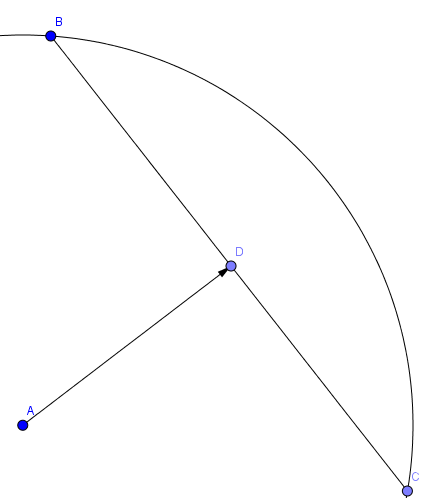
\includegraphics[width=0.3\linewidth]{images/quatrot1} 
	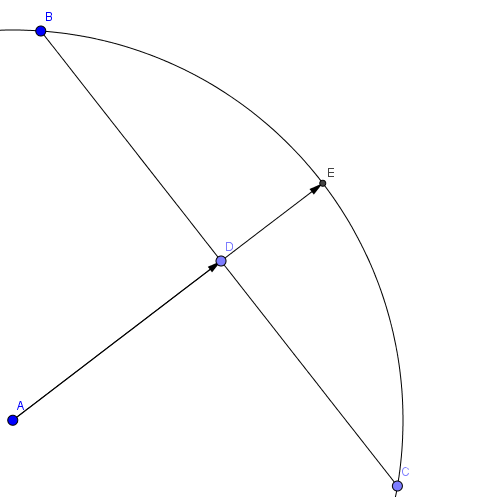
\includegraphics[width=0.33\linewidth]{images/quatrot2} 
	\caption{\label{fig:image} On the left: Idea, how linear interpolation between rotation matrices looks. If linear interpolation between two points on a circle is used, the resulting points do not lie on the circle. On the right: Interpolating with quaternions. The result can be easily mapped onto the sphere by normalizing the quaternion.
	}
\end{figure}



\marginpar{Ist das hier okay, dass ich die Notation der Matritzen missbrauche? Der erste Parameter der Rotationatrix ist ja eigentlich, welches Element eines Quaternions verwendet wird, aber aus der Notation wird denke ich klar, dass statdessen der einem Beispiel zugeordnete quaternion gemeint ist.}

\subsection{Recap Skinning}
Now we have a method to deform meshes with the help of bones and to blend in given example poses.
The input consists the constant data:
\begin{itemize}
\item The Vertex positions in undeformed state: $\bm u\in\mathbb{R}^{N\times 3}$
\item The weighting of each bone for the vertcies: $\bm W\in\mathbb{R} ^{N \times B}$
\item The transformation for each example pose, consiting of
	\subitem The rotational part $\bm R\in\mathbb{R}^{B\times 4\times  E}$
	\subitem The translational part $\bm T\in\mathbb{R}^{B \times 3\times E}$
\end{itemize}
and the changing data:
\begin{itemize}
	\item example Weights $\bm{E}\in\mathbb{R}^{N\times E}$
\end{itemize}
Let $\text{rotate} (\bm{q},\bm{x})$ be the function that rotates the position $\bm{x}$ by the quaternion $\bm{q}$.
The skinned mesh vertex positions $\bm{x} \in \mathbb{R}^{N\times 3}$ can now be calculated by:
\begin{align}
\bm{x}_i = \sum_{b\in B} \bm{W}_{ib}\left(\sum_{e=1}^{E}\bm{E}_{ie}\bm{T}_{be} + \text{rotate}(\text{QLERP}(\bm{E}_i,\bm{R}_b),\bm{u}_i)\right)
\end{align}
